\documentclass{article}

\usepackage[utf8]{inputenc}
\usepackage[swedish]{babel}
\usepackage{color}
\usepackage{listings}
\usepackage{hyperref}
\usepackage[a4paper, margin=2.8cm]{geometry}
\usepackage{graphicx}
\hypersetup{
    colorlinks=true, %set true if you want colored links
    linktoc=all,     %set to all if you want both sections and subsections linked
    linkcolor=black,  %choose some color if you want links to stand out
}


\definecolor{codegreen}{rgb}{0,0.6,0}
\definecolor{codegray}{rgb}{0.5,0.5,0.5}
\definecolor{codepurple}{rgb}{0.58,0,0.82}
\definecolor{backcolour}{rgb}{0.95,0.95,0.92}
 
\lstdefinestyle{mystyle}{
    backgroundcolor=\color{backcolour},   
    commentstyle=\color{codegreen},
    keywordstyle=\color{magenta},
    numberstyle=\tiny\color{codegray},
    stringstyle=\color{codepurple},
    basicstyle=\footnotesize,
    breakatwhitespace=false,         
    breaklines=true,                 
    captionpos=b,                    
    keepspaces=true,                 
    %numbers=left,                    
    numbersep=5pt,                  
    showspaces=false,                
    showstringspaces=false,
    showtabs=false,                  
    tabsize=2
}

\lstset{style=mystyle}

\author{Mattias Salo}
\title{Installation av Python}


\begin{document}

\pagenumbering{gobble}

\maketitle
\tableofcontents

\newpage
\pagenumbering{arabic}

\section{Windows}
\subsection{Ladda ner Python}
För att installera Python i Windows måste man ladda ner filerna från Pythons hemsida. \\
\url{https://www.python.org/downloads/windows/}\\
Ladda ner den senaste Python-versionen som börjar på 3, eftersom spelbiblioteket som ska användas kräver den versionen av Python.\\
\subsection{Installera Python}
Kom ihåg att du inte måste vara administratör på datorn för att installera Python.\\
\\
Starta installationen genom att dubbelklicka på den filen som har laddats ner från Pythons hemsida.\\
\begin{figure}[h!]
  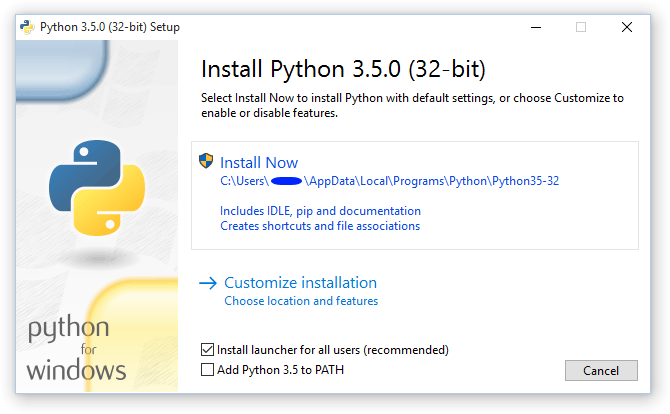
\includegraphics[width=\linewidth]{win_installer.png}
  \caption{Första installationsbilden}
  \label{fig:win}
\end{figure}\\
Välj "Install now"/"Installera nu"\ för att börja installationen av Python. Kryssa även i rutan "\ Add Python 3.X to PATH"\ för att enkelt kunna använda Python från Windows. Följ sedan installationsprogrammet genom att klicka OK eller nästa på alla frågor som kommer upp.
\subsection{Installera Pygame}
För att installera Pygame krävs det att man skriver någonting som liknar kod, starta kommandotolken genom att öppna start-menyn och skriv cmd, klicka sedan på enter. När kommandotolken är öppen ska detta skrivas in:
\begin{lstlisting}
py -m pip install -U pygame --user
\end{lstlisting}
Då ska kommer spelbiblioteket som vi kommer att använda för att skriva spel laddas ner. För att testa att pygame fungerar som det ska kan du prova ett exempel genom att skriva in
\begin{lstlisting}
py -m pygame.examples.aliens
\end{lstlisting}
om detta fungerar så har Pygame installerats ordentligt och vi kan börja koda våra spel.

\section{Linux (Ubuntu)}
Ubuntu kommer förinstallerat med Python 3 så det enda som behövs göras är att installera Pygame. I nyare Ubuntu-installationer kan Pip behöva installeras (Pip är det progam som Python använder för att installera bibliotek). Detta görs enklast genom att installera pip med aptitude.
\begin{lstlisting}
sudo apt-get install pip3
\end{lstlisting}
Efter att Pip har installerats är det bara att installera Pygame.
\begin{lstlisting}
pip3 install pygame
\end{lstlisting}

\section{MAC OSX}
Att installera Python i MAC OSX kräver ett antal steg. 
\subsection{Installera XCode}
Det första som behöver göras är att installera \href{https://itunes.apple.com/us/app/xcode/id497799835?mt=12&ls=1}{XCode} genom Apples Appstore.
\subsection{Installera HomeBrew}
Det andra som behöver installeras för att kunna installera Python är att installera HomeBrew.\\
\textbf{Steg 1:} starta Terminalen\\
Gå till LaunchPad - other - terminal\\
\textbf{Steg2:} Installera HomeBrew genom att skriva 
\begin{lstlisting}
/usr/bin/ruby -e "$(curl -fsSL https://raw.githubusercontent.com/Homebrew/install/master/install)"
\end{lstlisting}
i terminalen och klicka på enter.\\
\\
Skriv sedan in de tre följande kommandonen efter varandra, de två senare kan ta lång tid att fullfölja men ha tålamod och skriv in dem en efter en.
\begin{lstlisting}
echo export PATH='/usr/local/bin:$PATH' >> ~/.bash_profile
brew update
brew doctor
\end{lstlisting}
\subsection{Installera Python 3}
Installera Python genom att skriva 
\begin{lstlisting}
brew install python3
\end{lstlisting}
i terminalen och klicka på enter.\\
\\
Nu är python 3 installerat.
\subsection{Installera Pygame}
För att installera pygame måste vissa andra paket installeras innan. Skriv in de tre kommandon som följer en i taget och klicka på enter mellan varje kommando.
\begin{lstlisting}
brew install mercurial
brew install sdl sdl_image sdl_mixer sdl_ttf smpeg portmidi
pip install hg+http://bitbucket.org/pygame/pygame
\end{lstlisting}

\end{document}
